\documentclass[../main.tex]{subfiles}
\begin{document}

\subsection{Artificial Neural Networks}
\label{sec:artificial-neural-networks}

\glspl{ann} were originally developed as a mathematical model of the biological brain
(\cite{McCulloch1943,Rosenblatt58theperceptron,Rumelhart1987}).
Although \glspl{ann} have little resemblance to real biological neurons, they are
a powerful \gls{ml} tool and one of the most popular research topics in the last years.
Nowadays, most researchers have shifted from the prespective of the biological
neuron model to a more general \emph{function approximator} point of view;
in fact, it was proved that \glspl{ann} with enough capacity are capable of
approximating any measurable function to any desired degree of accuracy
(\cite{Cybenko1989,Hornik1991251}); this is, however, a non-constructive proof.

The basic structure of an \gls{ann} is a network of nodes (usually called neurons)
joined to each other by weighted connections.
Many varieties of \glspl{ann} have appeared over the years with different properties.
One important distinction is between \glspl{ann} whose connections form
feedback loops, and those whose connections are acyclic.
\glspl{ann} with cycles are typically referred to as recurrent neural networks
and those without cycles are known as \glspl{fnn}.

In this work, only \glspl{fnn} are used, in particular, a special kind that makes
use of the convolution operation called \glspl{cnn}.
The following section provides an overview of this networks as well as the
basic principles of training them.

\subsubsection{Convolutional Neural Networks}
\glspl{cnn} are a kind of \glspl{ann} particulary well-suited for computer vision
tasks. They were first introduced in \cite{LeCun1998} to perform the task of
hand-written digit classification and later popularized by \cite{Krizhevsky2012}
entry on the ImageNet Large Scale Visual Recognition Challenge 2012
(ILSVRC2012)\footnotemark, which won the classification task with a large
margin of 10\%.
\footnotetext{ILSVRC is a competition to estimate the content of
photographs for the purpose of retrieval and automatic annotation using a subset
of the large hand-labeled \href{http://image-net.org/}{ImageNet} dataset
(around 10,000,000 labeled images depicting 10,000+ object categories) as
training. In the classification task, the algorithms are evaluated by the error
rate in the test images presented with no initial annotation.}

A \gls{cnn} consist of an input and an output layer, as well as multiple hidden
layers (see figure \ref{fig:alexnet}). The input layer contains the data
(e.g., RGB image) with minimal preprocessing (normalization, cropping...),
in contrast to other \gls{ml} algorithms that need hand-engineered features.
The output layer is different depending on the task.

Each hidden layer performs the convolution operation with one or more
filters (commonly refered to as kernels by the \gls{dl} community) taking the
previous layer's output as the input and then an element-wise
non-linear function is applied to the output.
The non-linearities allow the model to extract
hierarchical features (early layers extract the called low-level features
and deeper layers extract high-level features)
from the input data as it is illustrated in figure
\ref{fig:cnn-visualization} on page~\pageref{fig:cnn-visualization}
extracted from \cite{Zeiler2014}.

Down-sampling (also known as pooling in the \gls{dl} literature) is also a very
common operation applied after some hidden layers, aimed to make the model
tranlation-invariant and reduce memory needs.
Three main methods can be used to represent the set of
$N$ (or $N \times N$) neighbouring samples with a single number:
\begin{enumerate*}[label=\itshape\alph*\upshape)]
\item Max-pooling uses the maximum value;
\item The average value is used by the average-pooling method and
\item Standard decimation ``takes'' a sample out of every $N$ samples,
it is usually implemented via $N$-strided (skipping $N - 1$ positions when
sliding the filter) convolution to compute only the used values.
\label{n-strided-conv}
\end{enumerate*}

Other kinds of layers like dropout (\cite{Srivastava2014})
and batch-normalization (\cite{Ioffe2015}) can be used for regularization
or faster training process.

\begin{figure}[h]
\centering
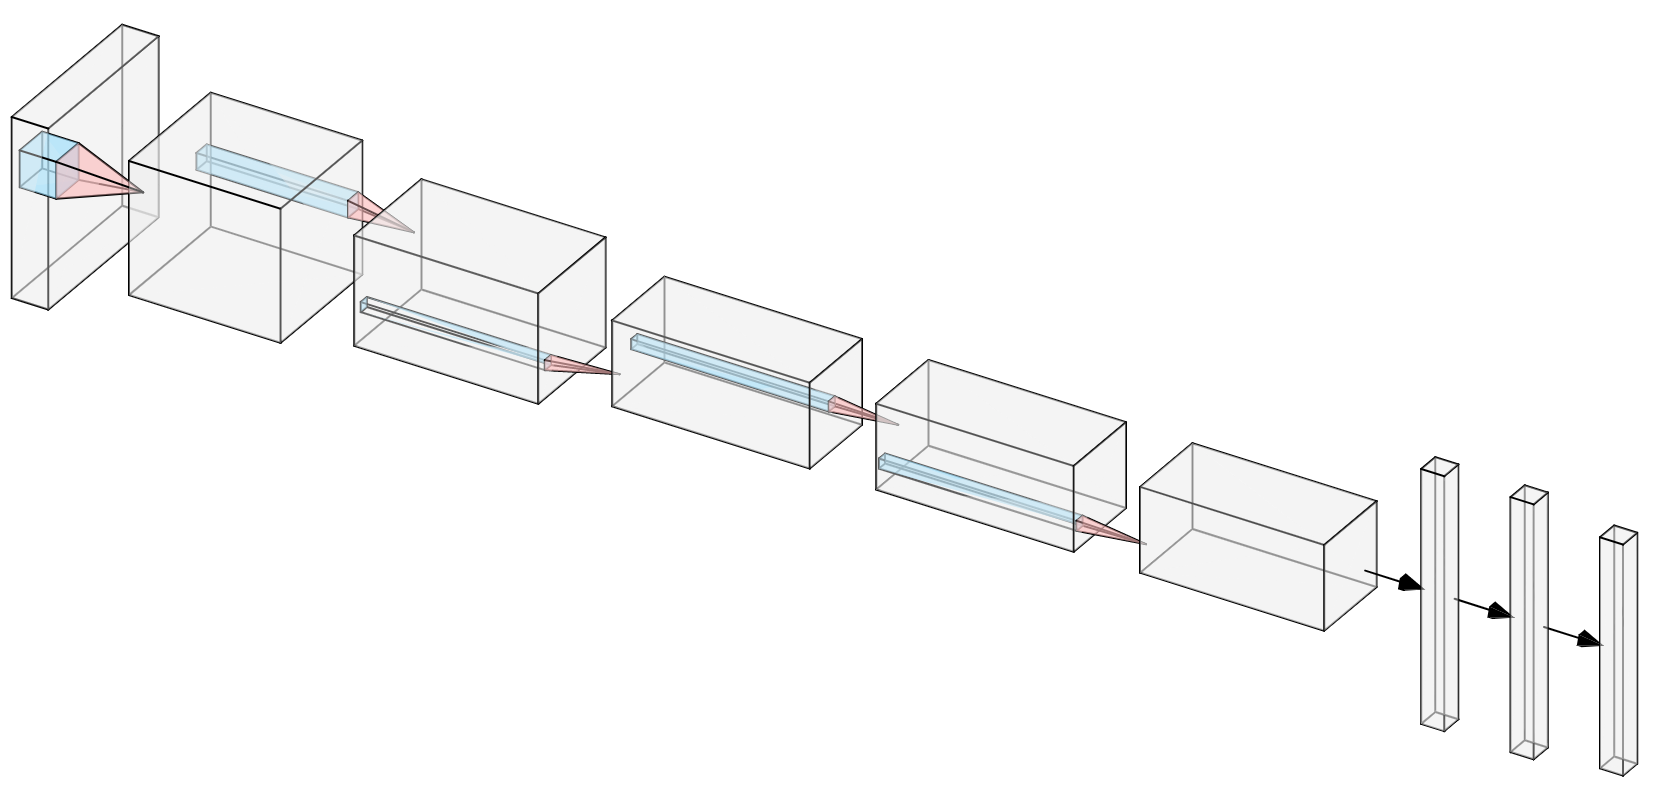
\includegraphics[width=.7\linewidth]{nn}
\caption{Visualization of a CNN with five convolutional layers and two
fully-connected layers (a kind of layer not described in this work).}
\label{fig:alexnet}
\end{figure}

\begin{figure}[h]
\centering
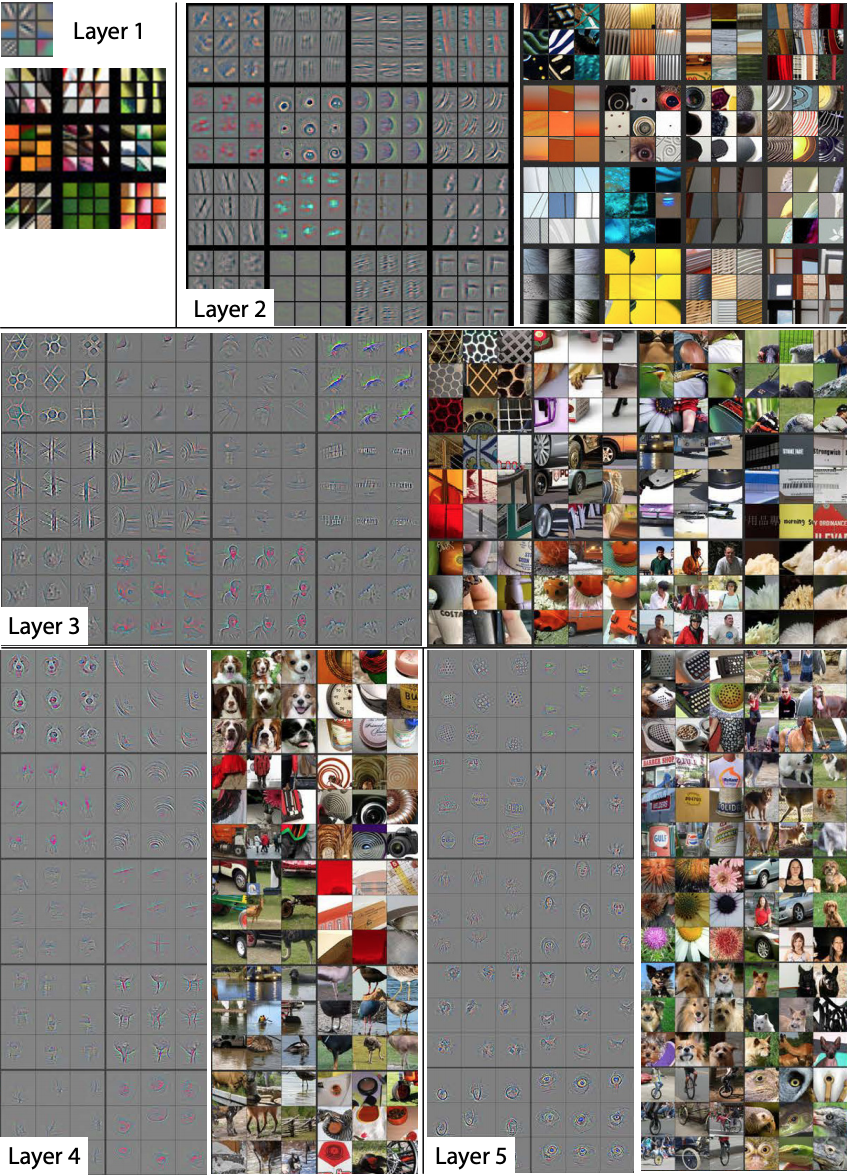
\includegraphics[width=.9\linewidth]{CNN_visualization}
\caption{Visualization of features in a fully trained model.
For layers 2-5 the top 9 activations in a random subset of feature maps are shown
projected down to pixel space using the ``deconvolutional'' network introduced in
\cite{Zeiler2014} work}
\label{fig:cnn-visualization}
\end{figure}

\subsubsection{Training artificial neural networks}\label{sec:optimizers}
Finding (or learning) the best set of parameters ($\theta$) (weights, filters,
...) of a network for a given problem can be posed as an optimization problem by
defining an appropiate objective function ($\mathcal{J}$).
In a supervised setting, where training data composed by
inputs (\textbf{X}) and targets (\textbf{Y}) is available:

\begin{equation}
\theta^* = \argmin_{\theta} \mathcal{J}
\left( (\tensor{X}, \tensor{Y}), f_{\theta} \right)
\end{equation}

The complex structure of \glspl{ann} makes this optimization problem non-convex,
hence iterative methods are used for moving towards an optimum solution;
particulary, gradient descent based are the most common type as the networks
are ---by construction--- fully-differentiable.

The idea behind gradient descent is simple. Given a (random) initial value
for the input variables (e.g., filter coefficients in the case of \glspl{cnn}),
these are updated by moving towards the direction with greater slope
i.e., the gradient. Moving towards the direction of the gradient (gradient
ascent) will yield a local maximum, useful when maximizing the objective
function; while moving toward the direction oposite to the gradient will
yield a local minimum:
\begin{equation}\label{eq:gradient-descent}
\iteration{\theta_i}{n} \leftarrow \iteration{\theta_i}{n - 1}
- \mu \frac{\partial \mathcal{J}}{\partial \theta_i}
\rvert_{\iteration{\theta_i}{n - 1}}
\end{equation}
where the superscript $(n)$ denotes the $n$-th iteration step and $\mu$
(known as learning rate) controls how much the variables should change between
steps. Note that the length of the ``step'' is not only governed by the
learning rate but also by the magnitute of the gradient.

In a \gls{dnn} with thousands or millions of parameters, computing the partial
derivative with respect to each parameter independently is computationally restrictive.
In \cite{backprop} work, an algorithm to efficiently train \glspl{ann}
called backpropagation\footnotemark{}  which uses the principles of dynamic
programming and exploits the chain rule was presented and it is how almost
all \glspl{ann} are trained nowadays.
\footnotetext{This lead to the terminology of forward pass, when the output of
the model is computed sequentially from the input layer through each of the
hidden layers; and the backward pass, when the partial derivatives a computed
starting from the final layer and going back to the first hidden layer.}

\paragraph{Cost function} When training \glspl{ann}, the objective function is
commonly defined as a cost function with two parts: the expected value of a
loss plus a (weighted) regularization term.

\begin{subequations}\label{eq:cost-function}
\begin{align}
\mathcal{J}\left( (\tensor{X}, \tensor{Y}), f_{\theta} \right) & =
\mathbb{E}\{ L \left( f_{\theta}(\tensor{X}), \tensor{Y} \right) \}
+ \lambda R(f_{\theta}) \tag{\ref{eq:cost-function}}\\
& \approx \frac{1}{N}
\sum_{\tensor{x}_i, \tensor{y}_j \in \tensor{X}, \tensor{Y}}
{L \left( f_{\theta} (\tensor{x}_i), \tensor{y}_j \right)}
+ \lambda R(f_{\theta}) \label{eq:sgd}
\end{align}
\end{subequations}

Equation \eqref{eq:sgd} shows how the expected
value is approximated by taking the mean over $N$ samples (batch size) of the
dataset.
Stochastic gradient descent is the case where $N=1$, and mini-batch
gradient descent when $N$ is smaller than the total number
of samples in the dataset; a small batch size is almost mandatory for large
datasets, as computing the loss for every sample at each iteration step is very
time and memory expensive and not only that: a small batch size helps avoiding
bad local optima and improve generalization
(\cite{DBLP:journals/corr/abs-1804-07612,Zhang2017No0}).

The loss function will depend on our task. For example, in classification
problems with $c$ clases the cross entropy can be used:
$ L(\hat{\tensor{y}}_i, \text{y}_i) = -\log [\hat{\tensor{y}}_i]_{\text{y}_i},
\quad \text{y}_i \in \{0\ ..\ c - 1\}, \hat{\tensor{y}}_i \in \R^{c} $; this
loss enforces the model to make a good estimation of the class probabilities
given an input datapoint.
A loss function well aligned with our task is crucial, but defining such
mathematical description of some problems is not always straightforward.

\paragraph{Advanced gradient-based optimization methods}
The basic (stochastic/mini-batch) gradient descent methods tend to find bad
sub-optima when dealing with the noisy, non-convex landscape of \glspl{ann};
with a performance very sensitive to the initial values, learning rate and
batch size.
Many research work
(\cite{Adagrad,Hinton2012RMSProp,Zeiler2012ADADELTA,Kingma2014Adam})
has focused on this area, developing algorithms that try to
find better optima with fewer iterations. The one used in this work
is the Adam ``optimizer'' (\cite{Kingma2014Adam}) which defines the following
update rule based on adaptive estimates of gradient moments:

\begin{subequations}\label{eq:adam}

\begin{equation}
\iteration{\theta_i}{n} \leftarrow \iteration{\theta_i}{n-1} -
\mu \frac{\iteration{\hat{m}_i}{n}}{\sqrt{\iteration{\hat{v}_i}{n}} + \epsilon}
\tag{\ref{eq:adam}}
\end{equation}

\begin{equation} \label{eq:adam-m}
\iteration{\hat{m}}{n} \leftarrow \frac{\iteration{m}{n}}{1 - \beta_1^n},\quad
\iteration{m_i}{n} \leftarrow \beta_1 \iteration{m_i}{n-1} +
(1-\beta_1)\iteration{g_i}{n}
\end{equation}

\begin{equation} \label{eq:adam-v}
\iteration{\hat{v}_i}{n} \leftarrow \frac{\iteration{v_i}{n}}{1 - \beta_2^n},\quad
\iteration{v_i}{n} \leftarrow \beta_2 \iteration{v_i}{n-1} +
(1-\beta_2)\left(\iteration{g_i}{n}\right)^2
\end{equation}

\begin{equation}
\iteration{g_i}{n} \leftarrow
\frac{\partial \mathcal{J}}{\partial \theta_i}
\rvert_{\iteration{\theta_i}{n - 1}}
\end{equation}

\end{subequations}

The parameter update equation \eqref{eq:adam} looks similar to the one in
\eqref{eq:gradient-descent} but instead of directly using the gradient, its
based on the exponential moving average of the gradient ($\hat{m}$) with
a coefficient of $1 - \beta_1$ (equation \ref{eq:adam-m}) and the exponential
moving average of the squared gradient ($\hat{v}$) with a coefficient of
$1 - \beta_2$ (equation \ref{eq:adam-v}).
The $\beta$'s are refered to as momentum an typical values lie
around 0.9. $\epsilon$ is a small constant (e.g, $10^{-8}$) to provide numerical
stability when $\hat{v}_i$ is small.
The intuition behind this update rule is that the steps are forced
to be of size $\mu$, as we are dividing by the magnitude of the gradient; and
instead of taking the direction of the gradient at a given iteration step, the
gradient value is passed through a low-pass filter to avoid making sudden changes
that are common in stochatic optimization (specially with a small batch size).

\subsection{Generative Adversarial Networks}

In \gls{ml} generative models are ones which model the distribution of the data.
This models can be used to perform classification through the conditional
distribution (via a prior distribution of the classes) or to sample/generate
data. Multiple generative models have been proposed that make use of \glspl{dnn}
(\cite{Hinton2009,Kingma2013,Goodfellow2014}), \gls{gans} in particular have
gained a lot of attention as they are capable of generating realistic images.

\gls{gans} is a framework for estimating generative models via an adversarial
process, in which two models are trained: a generative model ($G$) that captures
the data distribution, and a discriminative model ($D$).

Both models are implemented as \glspl{dnn} (usually \glspl{cnn} in the case of
image data). $G_{\theta_g}(\tensor{z})$ maps from an input space of random
variables with distribution $p_z(\tensor{z})$ to data space.
$D_{\theta_d}(\tensor{x})$ outputs the
probability that $\tensor{x}$ came from the data distribution
$p_{data}(\tensor{x})$ rather than $G$. See figure \ref{fig:gan-diagram} for
a simple illustration.

$G$ is trained to minimize the likelihood of $D$ assigning a low probability
to its samples.
While $D$ is simultaneously trained to maximize the probability of assigning
the correct label to both training examples and samples from G.
Hence, the loss functions (see equation \eqref{eq:cost-function})
for each model are defined as (note how they go one against the other):

\begin{subequations}
\begin{equation}\label{eq:generator}
L_G = \log(1 - D(G(\tensor{z})))
\end{equation}

\begin{equation}\label{eq:discriminator}
L_D =
  \begin{cases}
    - \log(D(\tensor{x})), & \tensor{x} \sim p_{data} \\
    - \log(1 - D(\tensor{x})) \equiv - \log(1 - D(G(\tensor{z}))),
    & \tensor{x} \sim p_g
  \end{cases}
\end{equation}
\end{subequations}

Equivalently, $D$ and $G$ play the following two-player minimax game:
\begin{equation}\label{eq:gan-minmax}
\min_G \max_D \mathbb{E}_{x \sim p_{data}(x)}\{\log D(x)\} +
\mathbb{E}_{z \sim p_z(z)} \{\log(1 - D(G(z)))\}
\end{equation}

If $G$ and $D$ have enough capacity, they will reach a point at which both cannot
improve because $p_g = p_{data}$.
The discriminator will be unable to differentiate between the two distributions,
i.e. $D(x) = 0.5$.

\begin{figure}[H]
\centering
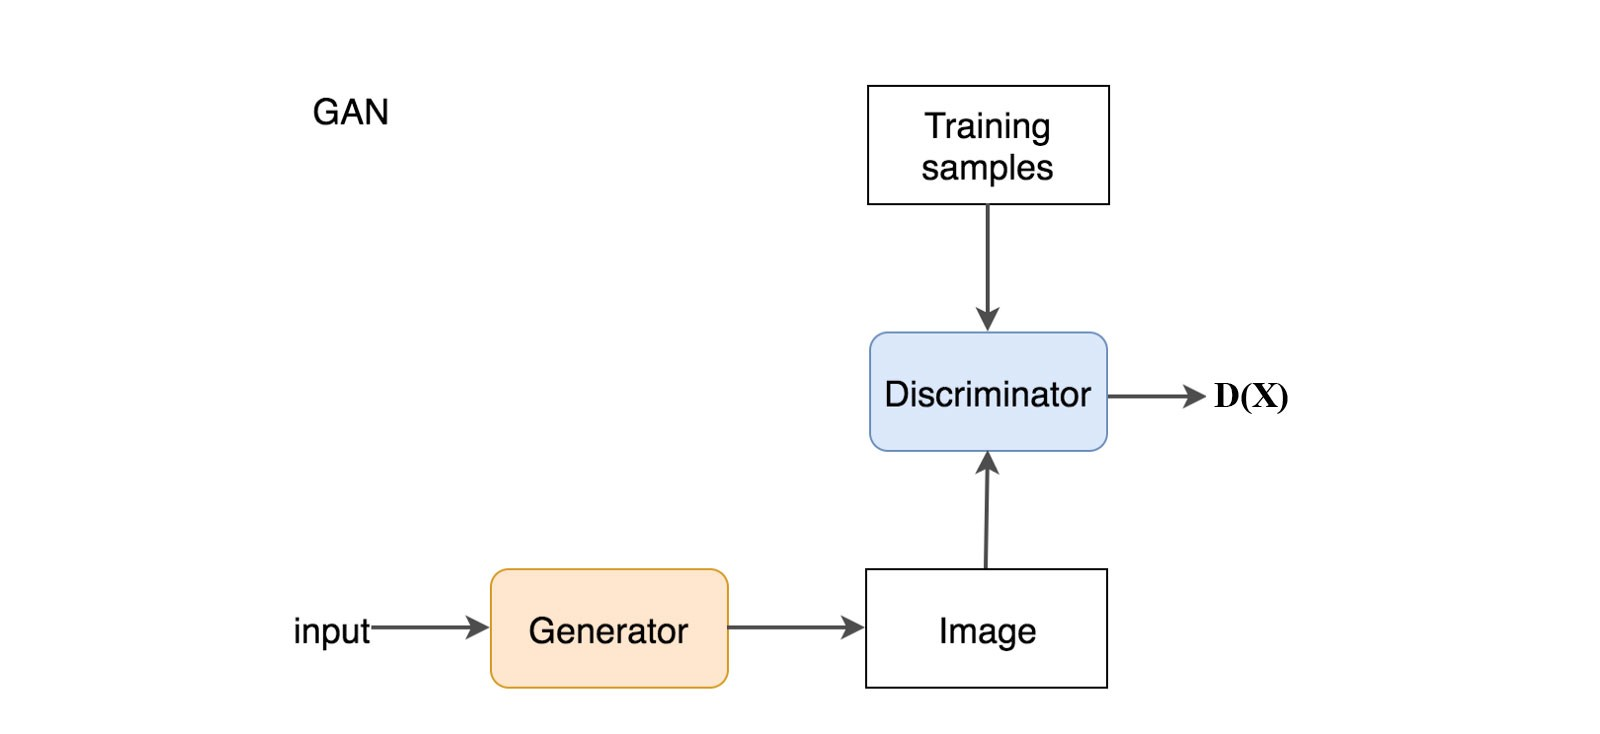
\includegraphics[width=.7\linewidth]{GAN-diagram}
\caption{Adversarial training process diagram}
\label{fig:gan-diagram}
\end{figure}

This way of traning a generative model is unstable and can fail to converge due
to a number of problems known as \emph{failure modes}:
\begin{itemize}
  \item Mode collapse: the generator collapses which produces limited varieties
  of samples,
  \item Diminished gradient: the discriminator gets too successful that the
  generator gradient vanishes and learns nothing,
  \item Unbalance between the generator and discriminator causing overfitting,
\end{itemize}

A number of publications
(\cite{Arjovsky2017,miyato2018spectral,DBLP:journals/corr/SalimansGZCRC16})
tackle this problems with architecture and loss function modifications, as well as
practical ``tricks''.
Successfully tranined generators, generate
very realistic samples as the constructed objective function essentially says
``generate samples that look realistic''.

\subsubsection{GANs for image-to-image translation}
\label{sec:gans-translation}

In this section, two frameworks for image-to-image translation based on \gls{gans}
are described. The first one, called pix2pix, (\cite{Isola2016}) uses a
conditional generative adversarial network to learn a mapping from input to
output images using paired data.
On the other hand, \gls{cyclegans} (\cite{Zhu2017a}) mapping is learned
without paired data.
Paired data consists of training examples
$\{\tensor{x}_i, \tensor{y}_i\}_{i=1}^N$
where correspondence between $\tensor{x}_i$ and $\tensor{y}_i$ exists, obtaining
this kind of data can be difficult (or impossible) and expensive; contrarily,
unpaired data consists of a source set $\tensor{X}$ and a target set $\tensor{Y}$
with no information provided as to which $\tensor{x}_i$ matches which
$\tensor{y}_i$ (if any).

\paragraph{Pix2Pix}
\cite{Isola2016} work presents a conditional adversarial setting and applies it
successfully to a variety of image-to-image translation problems that
traditionally would require very different loss formulations; proving that
\emph{learned loss functions} are versatile.
The losses used are similar to the ones in equations \eqref{eq:generator} and
\eqref{eq:discriminator}; but the discriminator not only gets the output of
the generator as input, but the corresponing input as well
(see figure \ref{fig:pix2pix} extracted from \cite{Isola2016}).
Apart from that, the generator is tasked to also be
near the ground truth in a L1 sense; this is done by modifying the generator's
loss function:
\begin{equation}
L_G = \log(1 - D(\tensor{x}, G(\tensor{x}))) +
\lambda \left\| \tensor{y} - G(\tensor{x}) \right\|_1
\end{equation}
\begin{figure}[t]
\centering
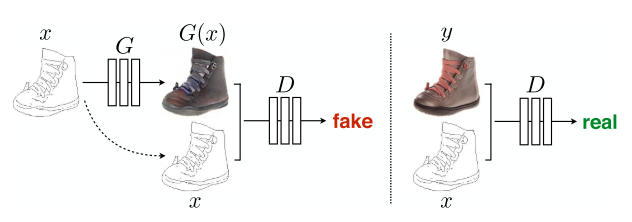
\includegraphics[width=.7\linewidth]{pix2pix-diagram}
\caption{Training a conditional GAN to map edges to photo.
The discriminator, $D$, learns to classify between fake and real {edge, photo}
tuples. The generator, $G$, learns to fool the discriminator.
Unlike an unconditional GAN, both the generator and discriminator observe the
input edge map.}
\label{fig:pix2pix}
\end{figure}

\paragraph{CycleGAN}
\cite{Zhu2017a} presents a method that builds on top of the Pix2Pix framework
for capturing special characteristics of one
image collection and transfering these into another image collection in the
absence of any paired training examples.
In theory, an adversarially trained generator can learn to map images from
a domain $X$ to look indistiguishable from images from a domain $Y$; 
in practice, it is difficult to optimize the adversarial objective in isolation
as this often leads to the mode collapse problem.
In \cite{Zhu2017a} work, this problem is addressed by adding more structure to the
objective; concretely, it ``encourages'' the mapping to be cycle-consistent, i.e.:
a function $\cycleGAN{X}{Y}$ that maps from domain $X$ to $Y$ should have and
inverse $\cycleGAN{Y}{X}$ that maps its output to the original input; as in
language translation, if a sentence is tranlated from Spanish to English and
then back to Spanish we should arrive to a sentence close to the original.
$ \cycleGAN{Y}{X}(\cycleGAN{X}{Y}(\tensor{x})) \approx \tensor{x} $.
This is done by simultaneously training two generators (with corresponding
discriminators $D_X$, $D_Y$ ---notice how in this case, these do not take the
source image as input---) and tasking them to not only ``fool'' their
discriminator but to also produce an image that is close to the original input
when translated back to the source domain (using the complementary generator),
this is done by defining the following losses for the generators
(more clearly visualized in figure \ref{fig:cyclegan}).\\
An aditional term called
idenity loss can be added to encourage the mapping to preserve color composition
between the input and the output by making the generator be near an idenity
mapping when samples from the target domain are provided.
Note that the input and output domains need to have the same number of channels.\\ The final losses for the generators are the following:
\begin{subequations}
\begin{equation}
\begin{split}
L_{\cycleGAN{X}{Y}} = &\log(1 - D_Y(\cycleGAN{X}{Y}(\tensor{x}))) \\
&+ \lambda_{cycle} \left\| \tensor{x} -
\cycleGAN{Y}{X}(\cycleGAN{X}{Y}(\tensor{x})) \right\|_1 \\
&+ \lambda_{identity} \left\| \tensor{y} - \cycleGAN{X}{Y}(\tensor{y}) \right\|_1
\end{split}
\end{equation}
\begin{equation}
\begin{split}
L_{\cycleGAN{Y}{X}} = &\log(1 - D_X(\cycleGAN{Y}{X}(\tensor{y}))) \\
&+ \lambda_{cycle} \left\| \tensor{y}
- \cycleGAN{X}{Y}(\cycleGAN{Y}{X}(\tensor{y})) \right\|_1 \\
 &+\lambda_{identity} \left\| \tensor{x} - \cycleGAN{Y}{X}(\tensor{x}) \right\|_1
\end{split}
\end{equation}
\end{subequations}
\begin{figure}[b]
\centering
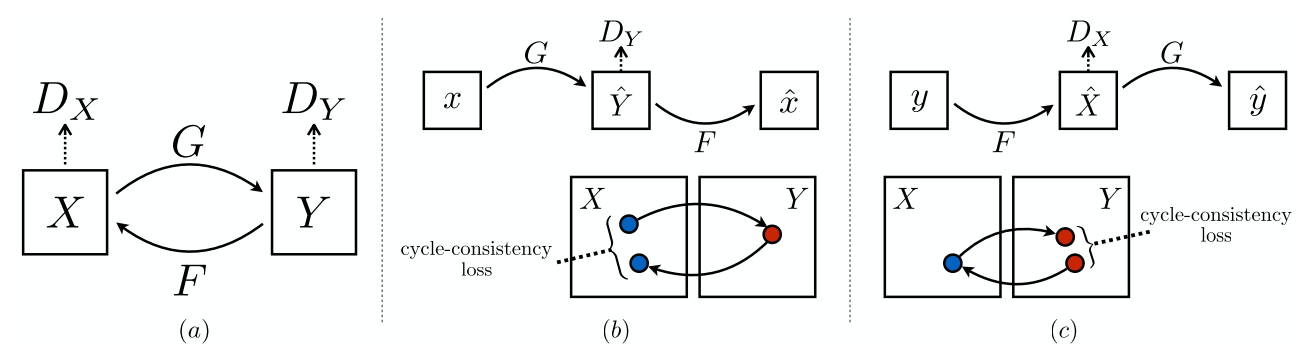
\includegraphics[width=.8\linewidth]{cyclegan-diagram}
\caption{(Extracted from \cite{Zhu2017a}) The mapping model denoted as $\cycleGAN{X}{Y}$ in this work is is
denoted in this figure as $G$ and $\cycleGAN{Y}{X}$ as $F$}
\label{fig:cyclegan}
\end{figure}

Note that neither Pix2Pix nor CycleGAN generators use a noise distribution
to generate samples (in contrast to the original \gls{gans} framework).
\end{document}
